\documentclass[note]{TechNote}
\usepackage[centertags]{amsmath}
\usepackage{amssymb,amsthm}
\usepackage[mathcal]{euscript}
\usepackage{tabularx}
\usepackage{cite}
\usepackage{c++}
\usepackage{tmadd,tmath}
\usepackage{caption}
\usepackage{subcaption}
\usepackage{algorithm}
\usepackage{algpseudocode}

%%---------------------------------------------------------------------------%%
\begin{document}

\refno{CSMD-00-000}
\subject{A Multilevel Monte Carlo Solver for Linear Systems}

\TIname{Mathematics and Computer Science Division}
\groupname{Computational Engineering and Energy Sciences Group}
\from{Stuart R. Slattery}
\date{\today}
\audience{
  \email{Stuart Slattery}{slatterysr@ornl.gov} \\
  \email{Tom Evans}{evanstm@ornl.gov} \\
  \email{Steven Hamilton}{hamiltonsp@ornl.gov}
}

%%---------------------------------------------------------------------------%%
\opening

\begin{abstract}
  Monte Carlo solvers for linear systems have been demonstrated to
  perform poorly for strongly elliptic problems. This poor performance
  is primarily due to the fact that both a large number of samples are
  required to obtain a good statistical error and that these samples
  require a large amount of time to compute. As a mechanism to reduce
  the computational complexity for such problems and thereby improve
  the figure of merit of the calculation, multilevel Monte Carlo has
  been introduced in finance problems, the solution of stochastic
  partial differential equations, and other algorithms that leverage
  Markov chain Monte Carlo. We adapt these ideas to form a multilevel
  Monte Carlo solver for linear systems which, in the form presented
  here, is effectively a stochastic realization of a geometric
  multigrid solver. Numerical studies indicate that the new multilevel
  method can reduce the time required to achieve a certain statistical
  error in the solution by at least two orders of magnitude, thereby
  dramatically reducing the computational complexity of the
  problem. Furthermore, the general formulation presented here
  indicates that this methodology is not restricted to geometric
  formulations of the multigrid method and could additionally be
  formulated using algebraic techniques.
\end{abstract}

%%---------------------------------------------------------------------------%%
\section{Introduction}
\label{sec:introduction}
Monte Carlo solvers for linear systems have been in existence for
decades as a stochastic alternative to iterative methods
\cite{forsythe_matrix_1950,wasow_note_1952,halton_sequential_1962,hammersley_monte_1964,spanier_monte_1969}. However,
these methods have failed to gain popularity both in the mathematics
and applications community partly due to their slow convergence bound
by the central limit theorem. Recent work has indicated that when used
as an acceleration in the Monte Carlo Synethetic Acceleration (MCSA)
method, exponential convergence rates may be achieved that are
competetive with contemporary iterative methods
\cite{evans_residual_2003,evans_monte_2009,evans_monte_2012,slattery_phd_2013}.
However, in this recent work it was discovered that for physics
problems that are largely elliptic (e.g. neutron transport in a light
water reactor), convergence of the Monte Carlo method is extremely
slow and prohibitive for the solution of larger systems. One avenue to
improve the time to solution for these calculations and to enable the
solution of more difficult problems is to study preconditioning
strategies as in \cite{slattery_phd_2013}. Another approach is to
instead focus on improving the time complexity of the Monte Carlo
sequence independent of the condition number of the linear problem.

Recent work in Monte Carlo methods for problems in finance and
stochastic partial differential equations has indicated that the
computationaly complexity of the problem can be dramatically reduced
by incorporating multigrid concepts into the solution scheme
\cite{heinrich_2001,giles_2008,cliffe_2011}. In this work, we adapt
those ideas and apply them to the Monte Carlo problem for linear
systems as a means of reducing the computational complexity of the
algorithm. To begin, we first introduce the elliptic model problem for
our numerical experiments and compare the spectral behavior of the
Monte Carlo method to traditional iterative smoothers that would be
used with the multigrid method. Next, we present the multilevel Monte
Carlo method for linear systems using a general algebraic
formulation. Finally, we present results using the model problem the
demonstrate the superiority of the multilevel method in terms of time
to solution.

%%---------------------------------------------------------------------------%%
\section{Monte Carlo Solver Fourier Analysis}
\label{sec:fourier_analysis}
We would first like to analyze the behavior of Monte Carlo solvers in
the context of error modes for a given model problem with the
numerical analysis presented here closely following that presented in
\cite{briggs_multigrid}. For this analysis, we will use the following
one-dimensional, homogenous model problem:
\begin{equation}
  \nabla^2 x = 0\:.
  \label{eq:model_problem}
\end{equation}
We discretize the problem into $N$ discrete points
where now $\ve{x} \in \mathbb{R}^N$ with boundary conditions:
\begin{equation}
  \ve{x}_1 = 0,\ \ \ve{x}_N = 0\:.
  \label{eq:boundary_conditions}
\end{equation}
The Laplacian is discretized using a standard second-order finite
difference with a grid spacing of one:
\begin{equation}
  (\nabla \ve{u})_i = \ve{u}_{i-1} - 2 \ve{u}_{i} + \ve{u}_{i+1}\:,
  \label{eq:discrete_laplacian}
\end{equation}
which then gives the following linear problem:
\begin{equation}
  \ve{A}\ve{x} = \ve{0}\:.
  \label{eq:linear_problem}
\end{equation}
To bound the spectral radius of the problem we will use a Jacobi
preconditioner:
\begin{equation}
  \ve{M} = diag(\ve{A})\:,
  \label{eq:preconditioner}
\end{equation}
such that we instead solve the following linear problem:
\begin{equation}
  \ve{M}^{-1}\ve{A}\ve{x} = \ve{0}\:.
  \label{eq:precond_problem}
\end{equation}
To elucidate the effect of a given solution technique on a given error
mode in the problem, we can assign an initial guess of $\ve{x}^0$ to
be a chosen Fourier mode:
\begin{equation}
  \ve{x}^0_i = \sin\Bigg( \frac{ik\pi}{N} \Bigg)\:,
  \label{eq:fourier_mode}
\end{equation}
where $\ve{x}^0_i$ is the $i^{th}$ component of the initial guess and
k is the wave number of the chosen Fourier mode. 

Monte Carlo solvers are effectively a stochastic realization of
Richardson's iteration and therefore we will first look at the
performance ofRichardson's iteration as a smoother:
\begin{equation}
  \ve{x}^{k+1} = (\ve{I}-\ve{M}^{-1}\ve{A})\ve{x}^k\:,
\end{equation}
where $k$ is the iteration index and which is equivalently a Jacobi
iteration when Jacobi preconditioning is
used. Figure~\ref{fig:richardson} gives infinity norm of the error in
the solution vector\footnote{The solution to the homogenous problem is
  zero and therefore $||\ve{e}||_{\infty} = ||\ve{x}||_{\infty}$.} as
a function of iteration for wave numbers of 1, 5, and 10 on a grid
with $G = 100$.
\begin{figure}[h!]
  \begin{center}
    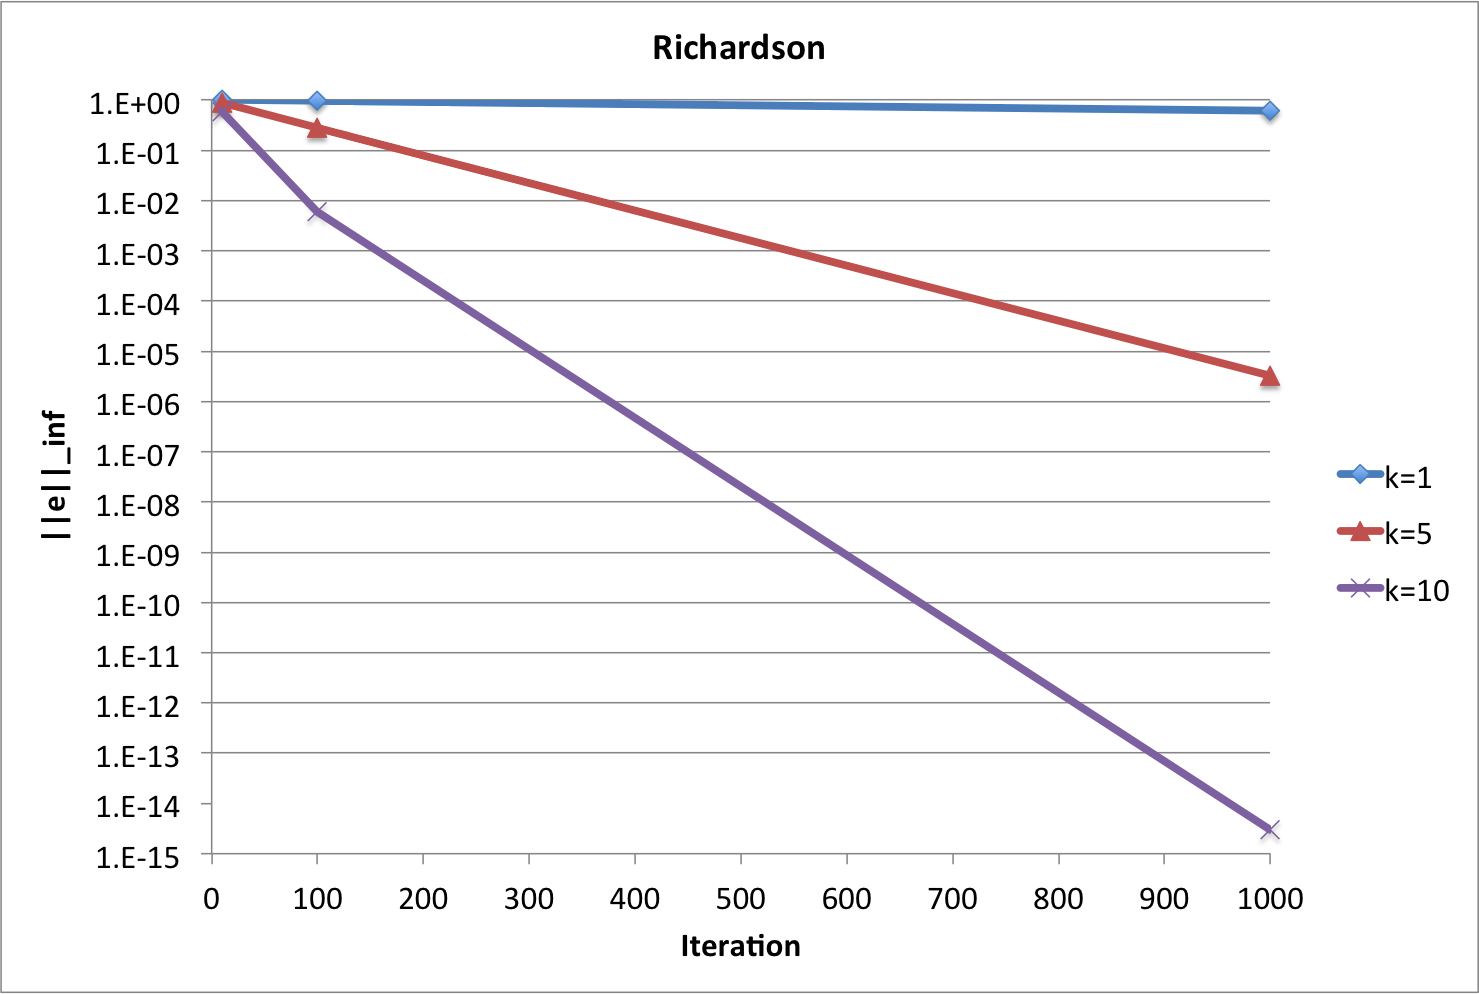
\includegraphics[width=5in]{richardson.png}
  \end{center}
  \caption{\textbf{Convergence of Richardson's iteration as a function
      of iteration for a grid of size $G = 100$.} \textit{Richardson's
      iteration performs better for larger wave numbers and therefore
      more oscillatory modes.}}
  \label{fig:richardson}
\end{figure}
Immediately we note that the larger the wave number the better
Richardson's iteration performs. Per the spectral analysis in
\cite{briggs_multigrid}, this iteration sequence perfoms better for
higher wave numbers as the eigenvalue spectrum spans a smaller space
then less oscillatory modes. This behavior motivates the multigrid
approach where moving a smooth mode to a coarser grid makes that mode
appear more oscillatory relative to that coarser grid, thus improving
convergence for that particular mode.

Next we perform the same calculations using the adjoint Monte Carlo
solver presented in \cite{evans_monte_2012}. Before doing this
however, we must first modify the linear problem as the Monte Carlo
solver is a direct method and therefore a homogenous problem with a
right hand side of $\ve{0}$ will yield no samples. Instead, we will
solve the residual problem:
\begin{equation}
  \ve{A}\ve{d} = \ve{r}\:,
  \label{eq:residual_problem}
\end{equation}
where the residual of the homogenous problem is:
\begin{equation}
  \ve{r} = -\ve{A}\ve{x}^0\:,
  \label{eq:homogenous_residual}
\end{equation}
and the solution is computed as:
\begin{equation}
  \ve{x} = \ve{x}^0 + \ve{d}\:.
  \label{eq:residual_solution}
\end{equation}
Forming the problem in this way lets us directly apply the adjoint
Monte Carlo method to the homogenous problem and then apply the
effective correction, $\ve{d}$, to the initial guess to give the
solution. This approach is also equivalent to performing a single
iteration of Halton's method \cite{halton_sequential_1962}. Using this
formulation we can again solve the model problem with wave numbers of
1, 5 and 10 on a grid of size $G = 100$ but this time we vary the
number of histories used to compute the solution instead of the number
of iterations. Figure~\ref{fig:adjoint_mc} gives the results of these
calculations.
\begin{figure}[h!]
  \begin{center}
    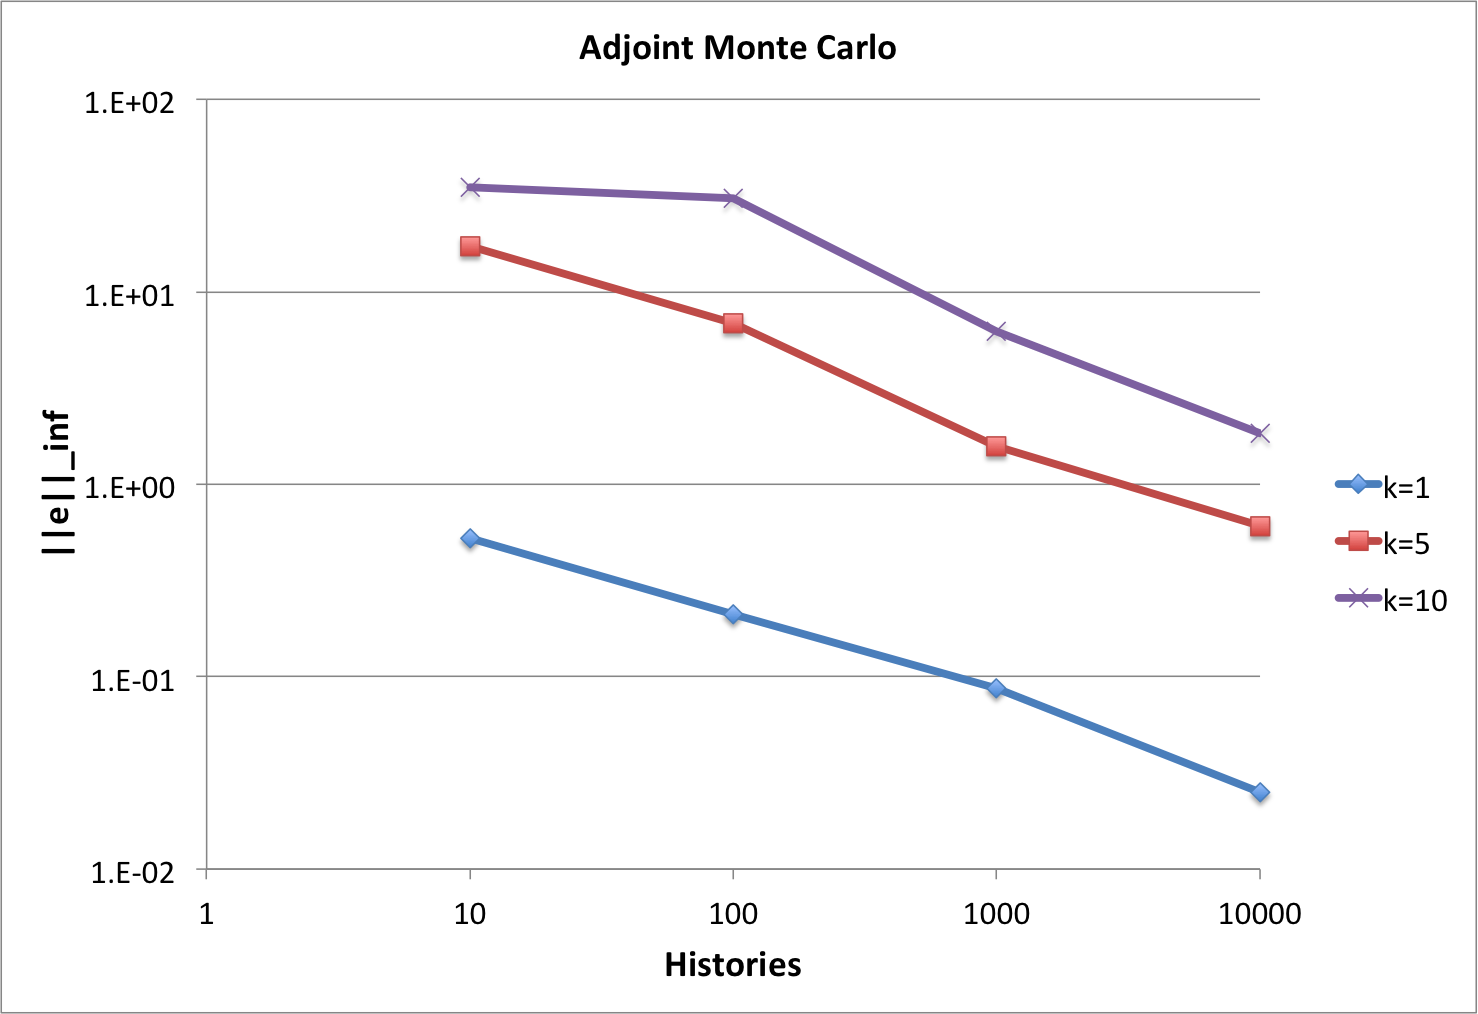
\includegraphics[width=5in]{adjoint_mc.png}
  \end{center}
  \caption{\textbf{Convergence of the adjoint Monte Carlo method as a
      function of sampled histories for a grid of size $G = 100$.}
    \textit{Adjoint Monte Carlo performs better for smaller wave
      numbers and therefore smoother modes.}}
  \label{fig:adjoint_mc}
\end{figure}
Surprisingly, the Monte Carlo method performs better for smooth modes
than more oscillatory modes\footnote{This behavior was also observed
  for the forward Monte Carlo method presented in
  \cite{evans_monte_2012}.}. The results of these calculations are
counterintuitive given the fact that the Monte Carlo solver is
effectively a stochastic realization of Richardson's iteration and
therefore one should expect the same spectral behavior from the
results.

Looking at the timing results in Table~\ref{tab:mc_timing}, we see
that the behavior of the Monte Carlo solver is in fact consistent with
these expectations.
\begin{table}[h!]
  \begin{center}
    \begin{tabular}{cc}\hline\hline
      \multicolumn{1}{c}{\textbf{Wave Number}} & 
      \multicolumn{1}{c}{\textbf{Time per History (s)}} \\
      \hline
      1 & 1 \\
      5 & 0.85 \\
      10 & 0.83 \\
      \hline\hline
    \end{tabular}
  \end{center}
  \caption{\textbf{Normalized average CPU time per history.}}
  \label{tab:mc_timing}
\end{table}
Timing results show that the average time required to compute an
entire history in the Monte Carlo solver decreases as a function of
wave number. We showed analytically in \cite{slattery_2013} that the
length of the random walk is equivalent to the number of Richardson
iterations that would be required to achieve a given convergence
criteria. In Figure~\ref{fig:richardson}, we see that fewer iterations
are required to converge larger wave numbers and therefore we should
also expect shorter random walks in the Monte Carlo solver and
therefore a faster time to solution as observed in
Table~\ref{tab:mc_timing}. However, this does not indicate why the
Monte Carlo solvers perform better for smoother modes rather than
oscillatory modes. Fortunately, the explanation for this behavior is
simple. Consider the plots for the Fourier modes with $k = 1$ and $k =
10$ given in Figure~\ref{fig:fourier_modes}.
\begin{figure}[h!]
  \centering
  \begin{subfigure}[b]{0.5\textwidth}
    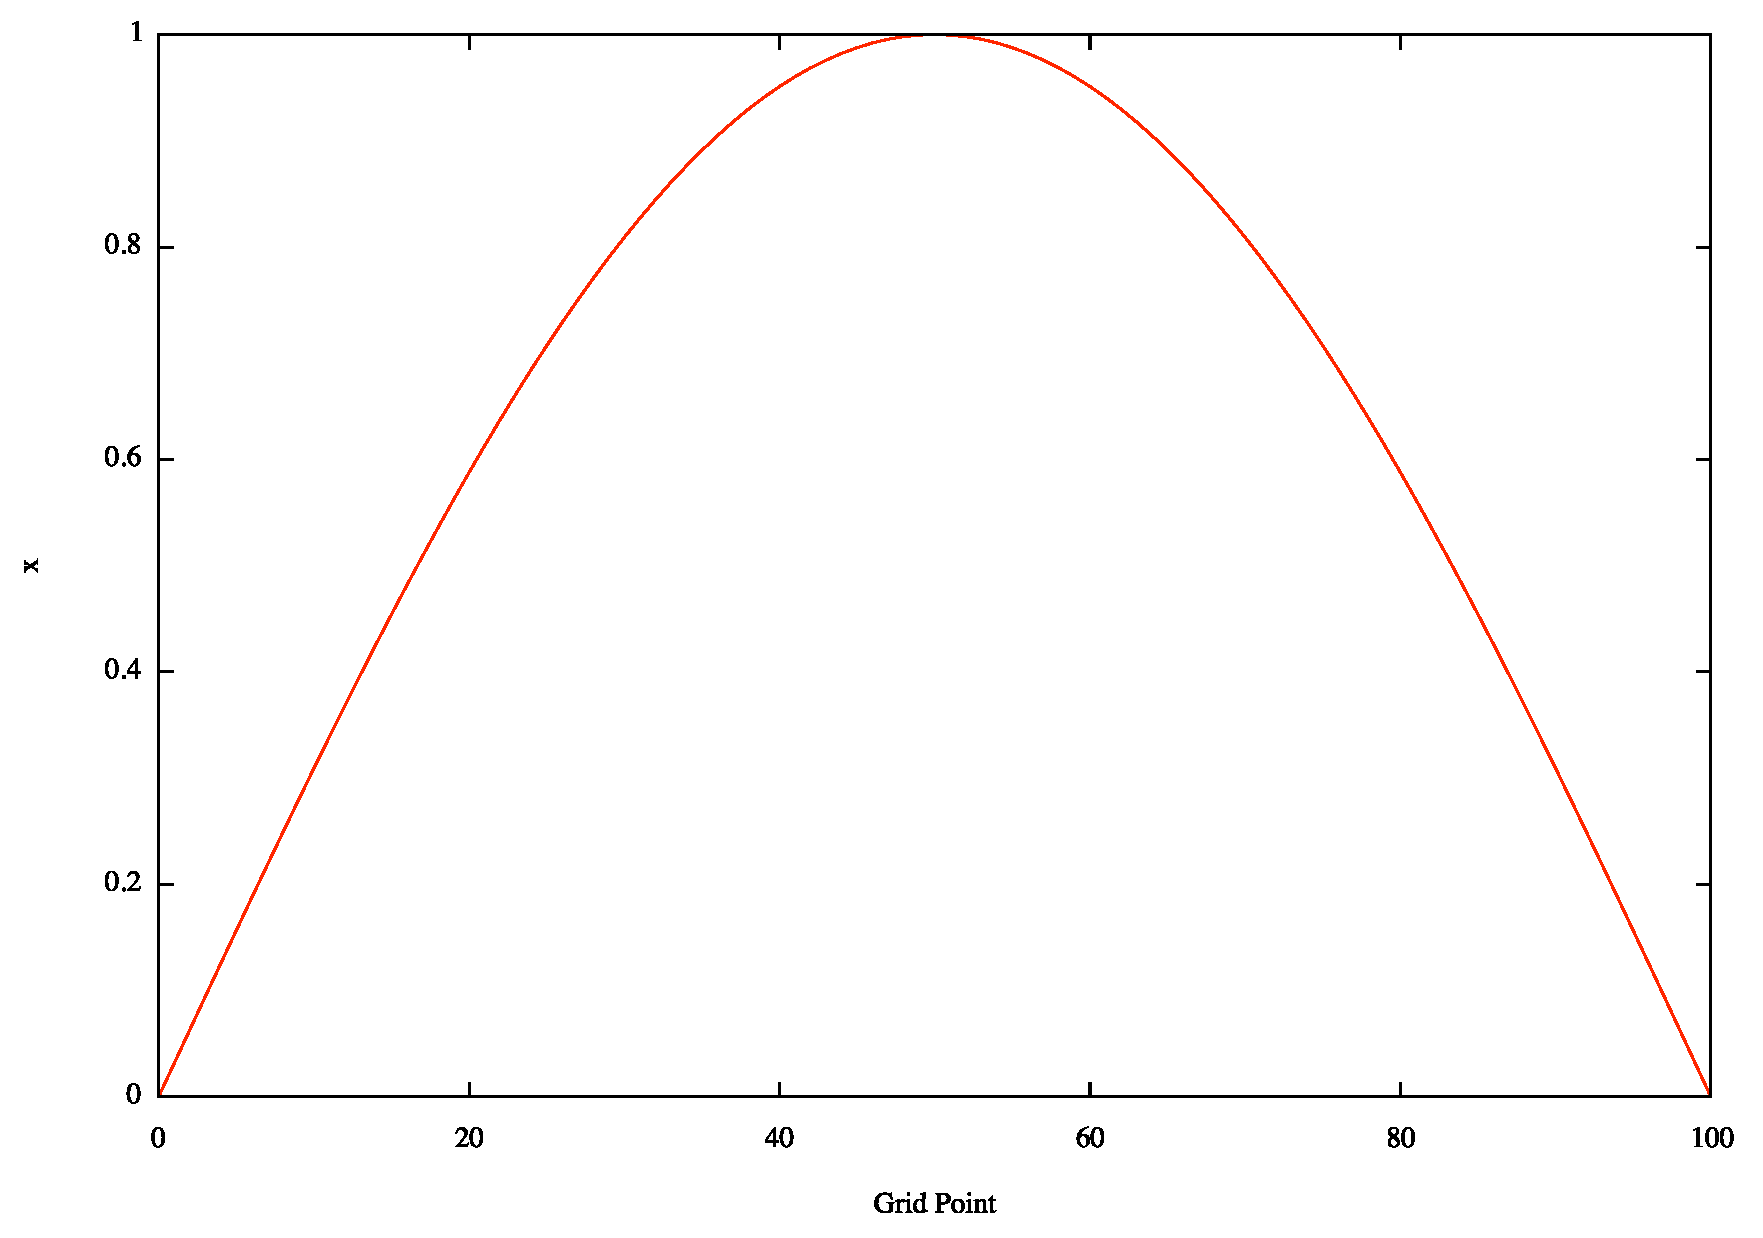
\includegraphics[width=\textwidth]{mode_1.pdf}
    \caption{\textbf{Fourier mode with $k = 1$.}}
  \end{subfigure}
  \begin{subfigure}[b]{0.5\textwidth}
    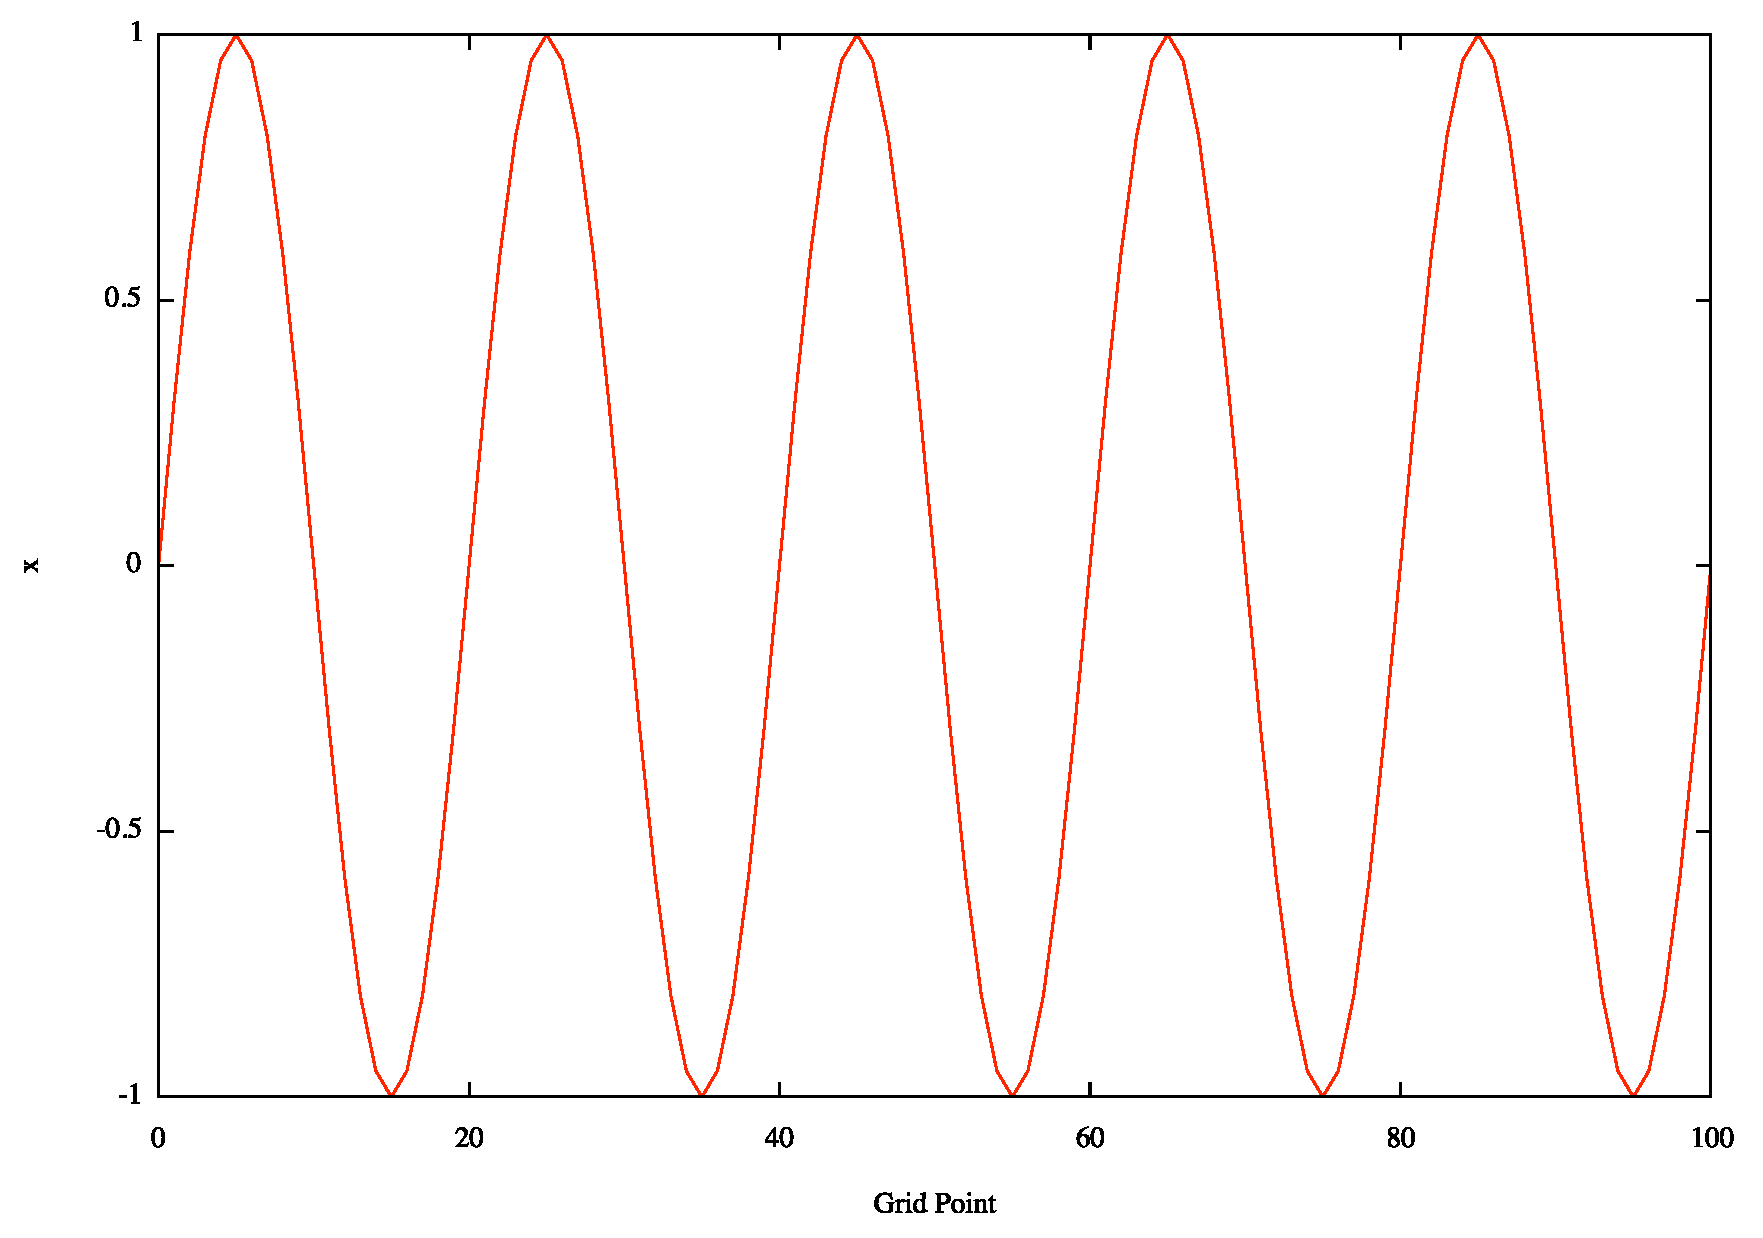
\includegraphics[width=\textwidth]{mode_10.pdf}
    \caption{\textbf{Fourier mode with $k = 10$.}}
  \end{subfigure}
  \caption{\textit{The more oscillatory the mode the finer the
      structure of the error. Finer structures require more samples to
      resolve them.}}
  \label{fig:fourier_modes}
\end{figure}
The higher the wave number is the more oscillatory the mode
appears. To resolve these fine structures in the error we therefore
naturally require more Monte Carlo samples to distinguish them from
one another.

Based on this, it may not seem that applying Monte Carlo in a
multigrid context will be useful considering that error modes appear
more oscillatory as the grid is coarsened. This would indicate that in
order to achieve the same amount of error on a coarse grid
representation of the problem, one would be required to compute many
more samples to resolve the resulting finer structures. However, we
may gain a computational advantage for two reasons. First, consider
the timing results in Table~\ref{tab:mc_timing}. As the error
structure becomes more oscillatory, the time it takes to compute a
sample decreases. Second, if we coarsen the grid the time it takes to
compute a sample will also decrease due to the decreased problem
size. Therefore, it is plausible that we might observe an improvement
in run times for the Monte Carlo problem by using a multigrid
approach.

%%---------------------------------------------------------------------------%%
\section{Multilevel Monte Carlo Algorithm}
\label{sec:algorithm}
A potential improvement in computational complexity motivates applying
techniques in multilevel Markov chain Monte Carlo recently developed
by Heinrich \cite{heinrich_2001} and Giles \cite{giles_2008}. We start
first with the standard Monte Carlo estimator for the $i^{th}$
component of the solution vector:
\begin{equation}
  \hat{\ve{x}}_i = \frac{1}{N} \sum_{m=1}^N x^m_i\:,
  \label{eq:standard_estimator}
\end{equation}
where $i \in [1,N]$, $N$ samples are made and $x^m_i$ is the $m^{th}$
observation. We next consider representing the problem in multiple
levels designated by $l$ with each one finer than the next such that
there are $L$ total levels and $l=L$ the coarsest level. We can
combine expectation values of the estimates from each of these levels
using the linearity of expectation such that:
\begin{equation}
  E(\ve{x}_{0}) = E(\ve{x}_{L}) + E(\ve{x}_{L-1} - \ve{x}_{L}) +
  E(\ve{x}_{L-2} - \ve{x}_{L-1}) + \dots + E(\ve{x}_{0} -
  \ve{x}_{(1)})\:,
  \label{eq:linearity_of_expectation}
\end{equation}
where $E(\ve{x}_{L})$ is the expectation value of the solution vector
at the coarsest level, $l = L$.  If we rewrite this summation as:
\begin{equation}
  E(\ve{x}_{0}) = E(\ve{x}_{L}) + \sum_{l=1}^L E(\ve{x}_{l} -
  \ve{x}_{l+1})\:,
  \label{eq:linearity_of_expectation_sum}
\end{equation}
we can then build a new \textit{multilevel estimator} for the $l^{th}$
level as:
\begin{equation}
    \hat{\ve{y}}_{l} = \frac{1}{N_l} \sum_{m=1}^{N_l} (x^m_{l} -
    x^m_{l+1})\:,
    \label{eq:level_estimate}
\end{equation}
where $N_l$ are the number of samples computed at the level and
$x^m_{l+1} = 0$ for $l=L$. Estimates from all levels can then be
combined to give the final solution as:
\begin{equation}
  \hat{\ve{x}} = \sum_{l=0}^L \hat{\ve{y}}_{l}\:.
  \label{eq:multilevel_estimator}
\end{equation}
It is critical to note here that the term $(x^m_{l} - x^m_{l+1})$
in Eq~(\ref{eq:level_estimate}) consists of observations from the same
Markov chain computed over the space of the $l^{th}$ level. 

Although multigrid methods for linear algebra problems indicate that a
coarsening parameter of $M = 2$ is optimal such that every level is
half the size of the finer level. However, Giles reports that values
of 4 and larger give optimal perfomance for these particular
estimators. In addition, as mentioned in
\S~\ref{sec:fourier_analysis}, because coarsening the problem makes
the modes appear more oscillatory, we therefore must compute more
samples at coarser levels to balance the error amongst the levels. For
this work we will use the result reported by Hienrich for computing
the number of samples at each level:
\begin{equation}
  N_l = M^{-3(L-l-1)/2}N\:.
  \label{eq:level_histories}
\end{equation}
It should be noted that Giles does not compute this quantity a priori
but instead first estimates the variance at each level and then
computes $N_l$ based on that variance.

Using the estimator given by Eq~(\ref{eq:multilevel_estimator}) we can
now define a multilevel Monte Carlo method for linear systems based on
the adjoint Monte Carlo solver given in \cite{evans_monte_2012}. To do
this, we must consider how to compute the expectation value
$E(\ve{x}_{l} - \ve{x}_{l+1})$ at each level in the problem. We are
required to construct observations on both grids from the same Markov
chain. Computing observations on the $l^{th}$ grid in this case is
simply the procedure for solving the adjoint Monte Carlo problem. In
this procedure we can simply tally observations on the grid for the
$l+1$ level through the use of a linear interpolation operator such
that a tally in some state of level $l$ is also a tally in some state
of level $l+1$ with that state determined by the linear operator such
that the weight of the observation is preserved. If this is the case,
then we can actually avoid tallying observations of the coarse grid
altogether and simply apply the linear interpolation operator the fine
grid results once all samples have been computed.

Using this idea we then define a \textit{prolongation operator},
$\ve{P}_{l+1}^l$, which maps a vector defined on grid $l+1$ to a
vector defined on grid $l$ and a \textit{restriction operator},
$\ve{R}_l^{l+1}$, which mpas a solution defined on grid $l$ to a
vector defined on grid $l+1$. We can then define the following
equivalent expecation value for a given level $l$:
\begin{equation}
  E(\ve{x}_{l} - \ve{x}_{(l+1)}) = \Big(\ve{I} - \ve{P}_{l+1}^l
  \ve{R}_l^{l+1}\Big) \hat{\ve{x}}_{l}\:,
  \label{eq:level_expectation}
\end{equation}
with $\hat{\ve{x}}_{l}$ given Eq~(\ref{eq:standard_estimator}) as the
solution on grid $l$ and where now the action of the restriction
operator maps the tally to the coarse level to compute the
observations on that grid and the action of the prolongation operator
on the coarse tally maps the result back to the fine
level. Eq~(\ref{eq:level_expectation}) then gives the following
multilevel Monte Carlo algorithm for linear systems now with arbitrary
right hand side vector, $\ve{b}$:
\begin{algorithm}[h!]
  \caption{Multilevel Adjoint Monte Carlo}
  \label{alg:mlamc}
  \begin{algorithmic}[1]

    \For{ l = 0...L }
    \State $\ve{A}_l \ve{x}_l = \ve{b}_l$
    \Comment{Solve the $l^{th}$ level problem with adjoint Monte
      Carlo}
    \If{ l != L }
    \State $\ve{x}_l = (\ve{I} - \ve{P}_{l+1}^l\ve{R}_l^{l+1}) \ve{x}_{l}$
    \Comment{Apply the multilevel tally}
    \EndIf
    \EndFor

    \For{ l = L...1 }
    \State $\ve{x}_{l-1} = ( \ve{I} + \ve{P}_{l}^{l-1} ) \ve{x}_{l}$
    \Comment{Collapse the tallies to the finest grid}
    \EndFor

  \end{algorithmic}
\end{algorithm}
This algorithm permits each of the levels to be computed independently
and then combined appropriately with the prolongation and restriction
operators. Like other multigrid algorithms for linear system, we are
required to produce a representation of the linear operator on each
level, $\ve{A}^l$, as well as the right hand side, $\ve{b}^l$. The
formulation of Algorithm~\ref{alg:mlamc} places no restrictions on the
form of $\ve{A}^l$, $\ve{b}^l$, $\ve{P}_{l+1}^l$, or $\ve{R}_l^{l+1}$
and therefore could be used with any multigrid scheme including those
arising from algebraic multigrid formulations.

%%---------------------------------------------------------------------------%%
\section{Results}
\label{sec:results}
To demonstrate the multilevel Monte Carlo algorithm we solve the
Poisson problem presented in \S~\ref{sec:fourier_analysis}, this time
with a grid of size $G = 1024$. For the coarsening parameter we will
first use a value of $M = 2$. In addition, we will introduce the
following standard figure of merit metric to assess the quality of the
Monte Carlo solver:
\begin{equation}
  FOM = \frac{1}{||\ve{e}||^2_{\infty} T}\:,
  \label{eq:figure_of_merit}
\end{equation}
where $||\ve{e}||_{\infty}$ is a measure of the variance of the
calculation and $T$ is the time required to solve the problem. The
larger the figure of merit, the more useful the solution scheme
is. For example, if two solutions schemes arrive at the same error but
the first calculation takes twice as long as the second, the figure of
merit will be twice as large for the second calculation.

We again perform calculations with initial guesses of wave numbers 1,
5 and 10 with Tables~\ref{tab:k1_results}, \ref{tab:k5_results}, and
\ref{tab:k10_results} giving the results of these calculations. In
these tables, the RFOM column indicates the relative figure of merit
which has been normalized to the single level calculation.
\begin{table}[h!]
  \begin{center}
    \begin{tabular}{cllll}\hline\hline
      \multicolumn{1}{c}{\textbf{Levels}} & 
      \multicolumn{1}{l}{\textbf{Samples}} & 
      \multicolumn{1}{l}{\textbf{$||\ve{e}||_{\infty}$}} & 
      \multicolumn{1}{l}{\textbf{Time (s)}} & 
      \multicolumn{1}{l}{\textbf{RFOM}} \\
      \hline
      1 & 10,000 & 0.022 & 119.1 & 1 \\
      2 & 13,535 & 0.026 & 72.0 & 1.14 \\
      3 & 14,785 & 0.035 & 33.2 & 1.38 \\
      4 & 15,226 & 0.039 & 13.7 & 2.63 \\
      5 & 15,382 & 0.027 & 5.5 & 13.86 \\
      6 & 15,437 & 0.036 & 2.3 & 19.21 \\
      7 & 15,456 & 0.045 & 0.98 & 28.00 \\
      8 & 15,462 & 0.081 & 0.41 & 20.66 \\
      9 & 15,464 & 0.267 & 0.17 & 11.72 \\
      \hline\hline
    \end{tabular}
  \end{center}
  \caption{\textbf{Multilevel Monte Carlo results for $k = 1$ with $M
      = 2$, $N = 10,000$ and run times reported in seconds.}}
  \label{tab:k1_results}
\end{table}
\begin{table}[h!]
  \begin{center}
    \begin{tabular}{cllll}\hline\hline
      \multicolumn{1}{c}{\textbf{Levels}} & 
      \multicolumn{1}{l}{\textbf{Samples}} & 
      \multicolumn{1}{l}{\textbf{$||\ve{e}||_{\infty}$}} & 
      \multicolumn{1}{l}{\textbf{Time (s)}} & 
      \multicolumn{1}{l}{\textbf{RFOM}} \\
      \hline
      1 & 10,000 & 0.668 & 101.6 & 1 \\
      2 & 13,535 & 0.381 & 60.0 & 5.21 \\
      3 & 14,785 & 0.396 & 28.0 & 10.34 \\
      4 & 15,226 & 0.599 & 11.9 & 10.64 \\
      5 & 15,382 & 0.638 & 4.7 & 23.60 \\
      6 & 15,437 & 1.052 & 1.8 & 23.15 \\
      7 & 15,456 & 1.070 & 0.67 & 59.16 \\
      8 & 15,462 & 1.180 & 0.23 & 144.10 \\
      9 & 15,464 & 2.130 & 0.10 & 99.95 \\
      \hline\hline
    \end{tabular}
  \end{center}
  \caption{\textbf{Multilevel Monte Carlo results for $k = 5$ with $M
      = 2$, $N = 10,000$ and run times reported in seconds.}}
  \label{tab:k5_results}
\end{table}
\begin{table}[h!]
  \begin{center}
    \begin{tabular}{cllll}\hline\hline
      \multicolumn{1}{c}{\textbf{Levels}} & 
      \multicolumn{1}{l}{\textbf{Samples}} & 
      \multicolumn{1}{l}{\textbf{$||\ve{e}||_{\infty}$}} & 
      \multicolumn{1}{l}{\textbf{Time (s)}} & 
      \multicolumn{1}{l}{\textbf{RFOM}} \\
      \hline
      1 & 10,000 & 1.81 & 98.6 & 1 \\
      2 & 13,535 & 1.67 & 59.6 & 1.94 \\
      3 & 14,785 & 2.41 & 27.1 & 2.05 \\
      4 & 15,226 & 3.20 & 11.5 & 2.74 \\
      5 & 15,382 & 1.85 & 4.93 & 19.14 \\
      6 & 15,437 & 3.89 & 1.95 & 10.95 \\
      7 & 15,456 & 3.79 & 0.78 & 28.68 \\
      8 & 15,462 & 7.08 & 0.30 & 21.62 \\
      9 & 15,464 & 11.7 & 0.11 & 21.45 \\
      \hline\hline
    \end{tabular}
  \end{center}
  \caption{\textbf{Multilevel Monte Carlo results for $k = 10$ with $M
      = 2$, $N = 10,000$ and run times reported in seconds.}}
  \label{tab:k10_results}
\end{table}

%%---------------------------------------------------------------------------%%
\bibliographystyle{ieeetr}
\bibliography{references}

\closing
\caution
\end{document}
